\begin{figure}[!tb]
	\centering
	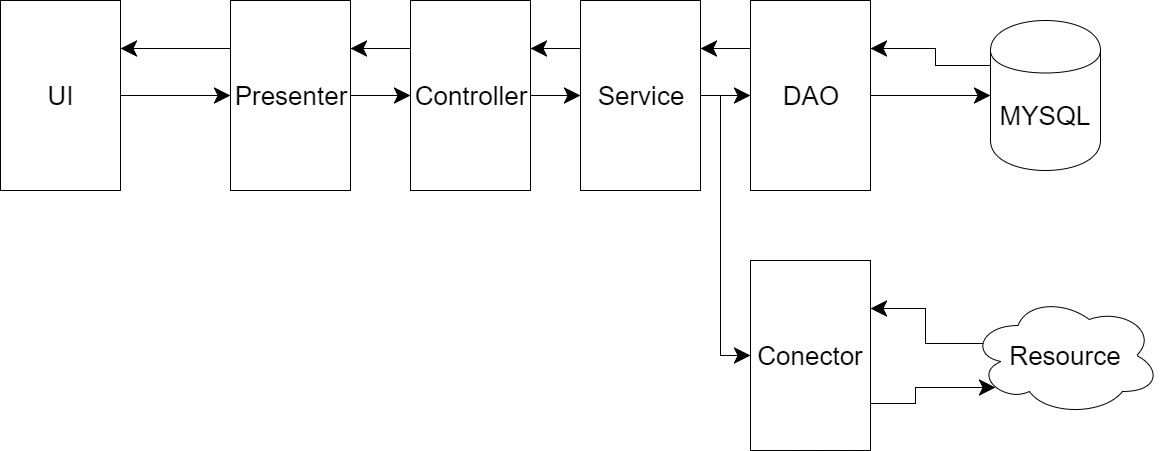
\includegraphics[width=\linewidth]{funcionamientoLuca.png}
	\caption{Arquitectura de LUCA}
    \label{fig:funcionamientoLuca}
\end{figure}

La Figura \ref{fig:funcionamientoLuca} muestra la arquitectura a alto nivel de \emph{LUCA}. \emph{LUCA} utiliza una arquitectura en capas, basada en la arquitectura inicial de \emph{Vaadin}. Se distinguen tres capas principales, propias de los sistemas empresariales: \emph{presentación}, \emph{negocio} y \emph{persistencia}.

La capa de \emph{presentación} se organizar de acuerdo con el patrón MVP y se genera automáticamente desde ficheros Java que describen la interfaz de usuario gracias al uso del framework \emph{Vaadin}.

La capa de \emph{negocio} se subdivide en dos subcapas: \emph{Access Control Layer} y \emph{Business Layer}. La primera subcapa se encarga de comprobar que quién realiza peticiones sobre la capa de negocio tiene los permisos y privilegios necesarios para ejecutar dichas acciones. Una vez otorgado dicho acceso, la petición se pasa a la capa de negocio propiamente dicha (\emph{Business Layer}), que es la que se encarga de actualizar los objetos del dominio de acuerdo con las reglas de negocio definidas. Para actualizar dichos objetos de dominio puede ser necesario recuperar ciertos elementos desde los sistemas donde se hallen almacenados, así como salvarlos en los mismos. Para realizar estas acciones, la capa de negocio se comunica con la capa de persistencia. 

La capa de \emph{persistencia} trata de ocultar los detalles de los diferentes sistemas donde se almacenan los datos a la capa de negocio, proporcionando una interfaz de alto nivel a través de la cual acceder a dichos datos. LUCA utiliza dos clases de sistema de almacemiento claramente diferenciados. 

Los datos propios de LUCA, tales como consultas existentes o usuarios creados, se almacenan en una base de datos relacional alojada en un gestor de bases de dato MySQL, al que se accede a través de una serie de clases DAO (\emph{Data Access Objects}). Además, LUCA necesita acceder a múltiples sistemas, de naturaleza diversa, para recuperar los datos de las consultas que ejecuta. Para facilitar el acceso a dichos sistemas, LUCA hace uso del concepto de \emph{conector}.

Un conector LUCA es un componente que se encarga de manejar la interacción con una datos de una fuente de datos externa. LUCA posee componentes genéricos por cada tipo de fuente a la que puede conectarse. De este modo, LUCA proporciona conectores para comunicarse son bases de datos relacionales alojadas en \emph{Oracle} a través de \emph{JDBC (Java DataBase Connectivity)}, servicios REST o servicios SOAP, entre otros. De este modo, cuando queremos incorporar una nueva fuente de datos a LUCA, simplemente deberemos instanciar un conector del tipo adecuado y configurarlo de manera adecuada para acceder a dicha fuente.







